\documentclass[cs4size]{ctexartutf8} 
\usepackage[unicode={true}]{hyperref}
\hypersetup{colorlinks,%
                 citecolor=black,%
                 filecolor=black,%
                 linkcolor=black,%
                 urlcolor=blue,%
                 pdftex}

\usepackage{graphicx}
\usepackage{float}

				
\title{脸脸应用需求方案}

\begin{document} 

\maketitle



\section{登录}

\begin{figure}[H]
\centering

\includegraphics[scale=0.5]{./1.png}
\label{p1}
\end{figure}

登录界面中,第一版可以只有新浪微博登录一种方式,第二版考虑添加腾讯微博等其它的登录方式。当用户量达到一定规模,首页可以增加一些总的统计数字:如总共有多少人摇了一摇等。

\section{首次登录-上传照片}

\begin{figure}[H]
\centering

\includegraphics[scale=0.5]{./2.png}
\end{figure}

上传照片时要以异步的方式在后台上传,不影响用户点完成。在此页面,附近的脸提供静态的虚拟脸即可,以刺激用户上传头像。当应用达到一定规模后,提供动态的附近的受欢迎的头像。

\begin{figure}[H]
\centering
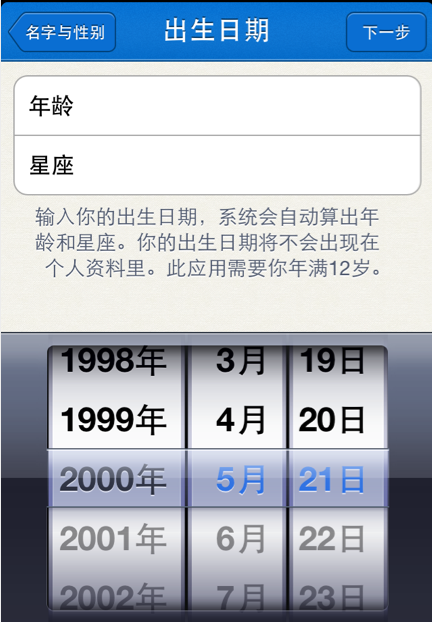
\includegraphics[scale=0.3]{./age.png}
\end{figure}

目前用户首次使用只需要上传照片,后期会考虑增加设置名字和出生日期这一步骤。


\section{现场}

\begin{figure}[H]
\centering

\includegraphics[scale=0.5]{./3.png}
\end{figure}


因为获取现场有时间延迟,所以在还未获得现场时,现场名称栏要显示转动的图标。获取现场成功后,图标停止。

因为经纬度有距离误差,所以现场的计算结果很可能不是用户真正的现场。因此用户需要能够手动选择目前所在的现场。


\section{关于摇一摇}
在现场摇一摇以后,就进入现场的群聊页面。摇一摇有多个功能,包括:给现场的所有人打招呼;在现场签到和确认当前的现场;如果商家有抽奖等活动,参与抽奖。

此外,在进入群聊页面后也可以摇一摇。此时的含义是参与商家发起的活动。


\section{现场群聊}

\begin{figure}[H]
\centering
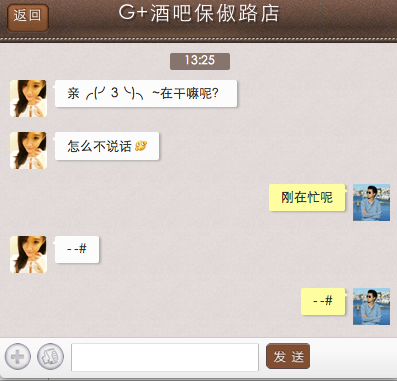
\includegraphics[scale=0.5]{./4.png}
\end{figure}

商家可以申请帐户绑定功能,将个人帐户与商家帐户绑定。比如商家的老板用自己的手机登录脸脸。此时,他登录脸脸后的发言会有单独的醒目的样式。商家帐户不能登录使用脸脸手机应用,只能登录脸脸网的商家管理后台。一个商家帐户可以绑定多个个人帐户。个人帐户采用新浪微博认证,商家帐户由脸脸网建立和管理。

现场群聊要给商家预留一行发布公告的地方。如果商家没有公告,此行自动隐藏。商家公告目前要在网站商家后台管理,以后考虑可以直接通过手机管理。

商家公告一般发布一些重要的、实效性在一天以上的信息。一些临时的信息可以在群聊页面用手机直接发布。


商家可以在群聊页面发起活动。比如主持人喊一二三,大家摇手机,摇到前10名的有奖。具体的活动规则由商家自行拟定。用户领奖时发一个确认信息给发起人即可。


\section{附近}

\begin{figure}[H]
\centering
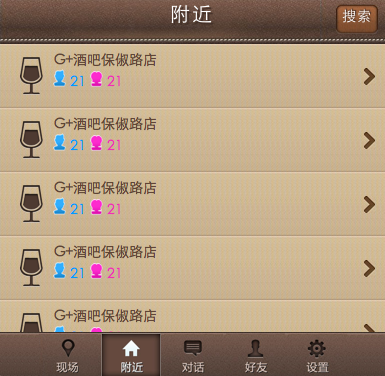
\includegraphics[scale=0.5]{./5.png}
\end{figure}

附近的商家默认按距离由近到远排序,要能按类别(酒吧、餐饮、活动等)筛选,按名称查询等。

附近的商家如果和用户当前的距离在1000米以内,可以进入该商家的现场,参与活动和发言。如果超过1000米,该用户只能查看该商家的信息。

附近的商家应该支持下拉获取更多数据功能和上拉刷新功能。所以类似的列表也都应该支持下拉和上拉操作。


\section{对话}

\begin{figure}[H]
\centering

\includegraphics[scale=0.5]{./6.png}
\end{figure}

对话应该包括两种类型:一种是个人之间的对话,一种是个人和组织的对话。两种对话要有不同的显示样式。个人在商家现场的群聊以及商家发送的信息以商家名义出现在会话中。系统通知消息应该出现在“脸脸”系统用户中。

初版聊天记录可以使用本地存储实现。后期需要实现用户更换手机后从服务器端同步聊天记录。


\section{个人聊天}

\begin{figure}[H]
\centering

\includegraphics[scale=0.5]{./7.png}
\end{figure}

个人聊天页面类似于群聊页面。其中聊天时支持的表情和动作还需要细化。点击摇一摇图标时,进入一个专门的摇一摇的界面,和微信类似。比如摇一摇的体验包括:动作 – 摇动;视觉 – 屏幕裂开并合上来响应动作; 听觉:有吸引力(男性是来福枪,女性是铃铛)的声音来响应动作;结果是发送一个消息。



\section{好友}

\begin{figure}[H]
\centering
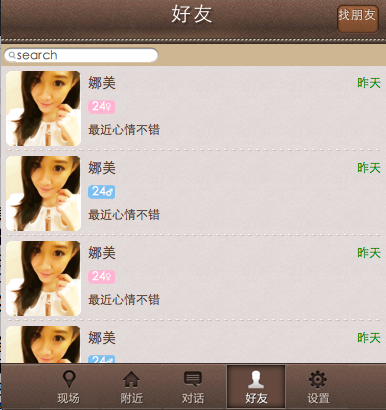
\includegraphics[scale=0.5]{./8.png}
\end{figure}

这里的好友是用户在脸脸上加的好友,且是单向关系(无需对方确认),和新浪微博没有关系。

找朋友目前要支持手机通讯录和从新浪微博好友两种来源。对于对方未加入脸脸的,可以发送邀请;对于已加入脸脸的,可以直接发送消息。

\section{个人信息}

\begin{figure}[H]
\centering
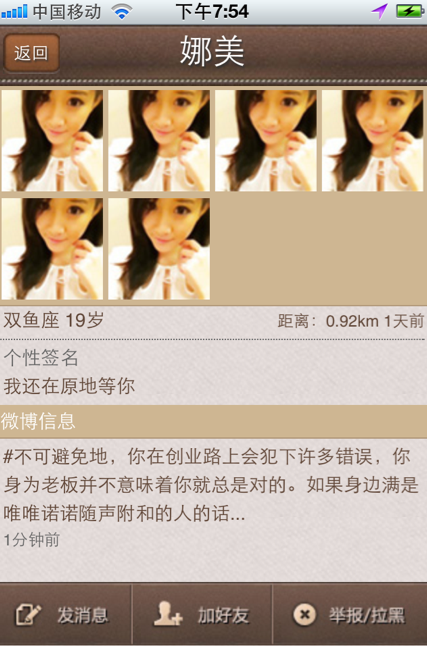
\includegraphics[scale=0.5]{./9.png}
\end{figure}

个人信息中的图片取自用户新浪微博中发的微博中的图片。距离改成地点。

\section{设置}

\begin{figure}[H]
\centering
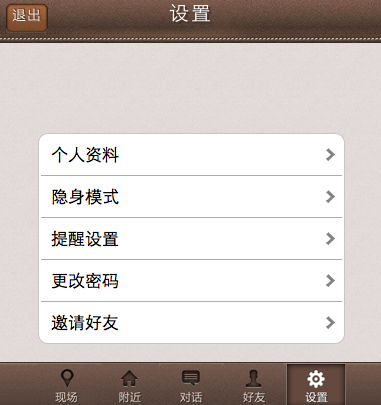
\includegraphics[scale=0.5]{./10.png}
\end{figure}

设置页面中,在菜单中要增加“退出”的功能,同时取消“修改密码”功能。“提醒设置”的功能要明确。有两种提醒,一种是系统消息,一种是好友在附近时的提醒。这两种提醒的实现机制不一样。系统消息采用应用内通知即可。好友在附近时的提醒最好是Push提醒,这样用户没使用脸脸时也能收到提醒。此外还需要有隐身功能和黑名单管理功能。



\newpage


\end{document}
